%%%%%%%%%%%%%%%%%%%%%%%%%%%%%%%%%%%%%%%%%
% Custom Class
% LaTeX Template
% Version 1.0 (28/2/15)
%
% This template has been downloaded from:
% http://www.LaTeXTemplates.com
%
% Original author:
% Vel (vel@latextemplates.com)
%
% License:
% CC BY-NC-SA 3.0 (http://creativecommons.org/licenses/by-nc-sa/3.0/)
%
%%%%%%%%%%%%%%%%%%%%%%%%%%%%%%%%%%%%%%%%%

%----------------------------------------------------------------------------------------
%	DOCUMENT SPECIFICATIONS
%----------------------------------------------------------------------------------------

% Class options are specified in the square brackets before the class name
% The example class has two custom options: OPONE or OPTWO; one of these MUST be used or the compilation fails
\documentclass[OPONE]{example}
\usepackage{amsmath}
\usepackage{commath}
\usepackage{graphicx}
\graphicspath{ {./} }
%----------------------------------------------------------------------------------------

\begin{document}

%----------------------------------------------------------------------------------------
%	DOCUMENT CONTENT
%----------------------------------------------------------------------------------------

\noindent Question 3a - Exercise 4.1.3
\begin{list}{}{}
	
	\item {b.}  
	$f(x) = 1/(x^2-4)$ \hspace{.1 in}
	Not a function. If x is -2 or 2, 1/0 is not defined.

	\item{c.}  
	$f(x) = \sqrt{x^2}$ \hspace{.5 in}
	It is a function and is well-defined.
	

\end{list}

\noindent Question 3b - Exercise 4.1.5

	
\begin{list}{}{}
	
	\item{b.}	
	\{4, 9, 16, 25\}

	\item{d.}
	\{0, 1, 2, 3, 4, 5\}

	\item{h.}	
	\{(1,1), (2,1), (3,1), (1,2), (2,2), (3,2), (1,3), (2,3), (3,3)\}
	
	\item{i.}	
	\{(1,2), (1,3), (1,4), (2,2), (2,3), (2,4), (3,2), (3,3), (3,4)\}
	
	\item{l.}	
	\{ $\emptyset$, \{2\}, \{3\}, \{2, 3\} \}
	
\end{list}


\newpage
\noindent Question 4 I. a - Exercise 4.2.2

\begin{list}{}{}

	\item{c.}
	$h: \textbf{Z}\rightarrow\textbf{Z}. \hspace{.1 in} h(x) = x^{3}$ \\
	 one-to-one \\
	 but not onto because for all $x$ in $\textbf{Z}$ there exists no $h(x) = 2$

	\item{g.}
	$f: \textbf{Z} \times \textbf{Z}\rightarrow \textbf{Z} \times \textbf{Z}, \hspace{.1 in} f(x, y) = (x+1, 2y)$ \\
	one-to-one \\
	but not onto because for all $(x,y)$ in $\textbf{Z}\times\textbf{Z}$ there exists no $f(x,y) = (1,1)$ 

	\item{k.}
	$f: \textbf{Z}^{+} \times \textbf{Z}^{+} \rightarrow \textbf{Z}^{+}, \hspace{.1 in}  f(x, y) = 2^{x} + y.$ \\
	not one-to-one because $f(0,2) = f(1,1) = 3$ \\
	and not onto because $f(x,y) = 0$ does not exist for $\textbf{Z}^{+} \times \textbf{Z}^{+} $

\end{list}


\noindent Question 4 I. b - Exercise 4.2.4

\begin{list}{}{}
	
	\item{b.}
	$f: \{0, 1\}^{3}\rightarrow\{0, 1\}^{3}.$ The output of f is obtained by taking the input string and replacing the first bit by 1, regardless of whether the first bit is a 0 or 1. For example, $f(001) = 101$ and $f(110) = 110$.\\
	not one-to-one because $f(000) = f(100) = 100$ \\
	and not onto because for all strings $x$ in $\{0, 1\}^{3}$ there is no $f(x) = 000$.
	
	\item{c.}
	$f:\{0, 1\}^{3}\rightarrow\{0, 1\}^{3}$. The output of f is obtained by taking the input string and reversing the bits. For example $f(011) = 110$.	 \\
	both one-to-one and onto
	
	\item{d.}
	$f: \{0, 1\}^{3}\rightarrow\{0, 1\}^{4}$. The output of f is obtained by taking the input string and adding an extra copy of the first bit to the end of the string. For example,$ f(100) = 1001$. \\
	one-to-one \\
	but not onto because for all strings $x$ in $\{0, 1\}^{3}$ there is no $f(x) = 1000$.
	
	\item{g.}
	Let A be defined to be the set \{1, 2, 3, 4, 5, 6, 7, 8\} and let B = \{1\}. $f: P(A) \rightarrow P(A)$. For $X \subseteq A, f(X) = X - B.$ Recall that for a finite set A, P(A) denotes the power set of A which is the set of all subsets of A. \\
	not one-to-one because for X = \{2, 3, 4\} and X = \{1, 2, 3, 4\}, f(X) = \{2, 3, 4\} \\
	and not onto because for any $X \subseteq A$, there is no solution to $F(X) = \{1, 2, 3, 4\}$
	
\end{list}

\noindent Question 4 II. \\

\noindent Give an example of a function on the set of integers to the set of positive integers  ($f: \textbf{Z} \rightarrow \textbf{Z}^{+}$) that is: 

\begin{list}{}{}
	
	\item{a.}
	one-to-one, but not onto \\	
	$f(x)$ = \begin{cases}	
	$-2x$ & \text{for $x < 0$} \\
	$2x + 3$ & \text{for $x\geq0$}
	\end{cases}

	\item{b.}
	onto, but not one-to-one \\
	$f(x) = \abs{x} + 1$
	
	\item{c.}
	one-to-one and onto \\
	$f(x)$ = \begin{cases}	
		$(\abs{x} \times 2) - 1}$ & \text{for $x < 0$} \\
		$(x \times 2) + 1$ & \text{for $x\geq0$}
	\end{cases}
	
	\item{d.}
	neither one-to-one nor onto \\
	$f(x) = x^{2} + 2$ will map any integer (positive or negative) to the positive set of integers, but not one-to-one as x = -1 and x = 1 both map to 3, nor onto as not all positive integers are the offsets of perfect squares
	
\end{list}
	

\newpage

\noindent Question 5a - Exercise 4.3.2

\begin{list}{}{}
	
	\item{c.}
	$f: \textbf{R} \rightarrow \textbf{R}$. & $f(x) = 2x + 3$	\\
	$f^{-1} (x) = \frac{x - 3}{2}$
	
	\item{d.}
	Let A be defined to be the set $\{1, 2, 3, 4, 5, 6, 7, 8\}$. $f: P(A) \rightarrow \{0, 1, 2, 3, 4, 5, 6, 7, 8\}$. For $X \subseteq A, f(X) = \abs{X}$. Recall that for a finite set A, P(A) denotes the power set of A which is the set of all subsets of A.	\\
	The function $f$ is not one-to-one, so $f^{-1}$ is not well-defined.
	
	\item{g.}
	$f: \{0, 1\}^{3} \rightarrow \{0, 1\}^{3}$. The output of $f$ is obtained by taking the input string and reversing the bits. For example, $f(011) = 110$. \\
	$f^{-1}(x)$ is obtained by taking the input string and reversing the bits.
	
	\item{i.}
	$f: \textbf{Z} \times \textbf{Z} \rightarrow \textbf{Z} \times \textbf{Z}, \hspace{.1 in} f(x, y) = (x+5, y-2)$ \\
	$ f^{-1}(x, y) = (x -5, y+2)$

\end{list}


\noindent Question 5b - Exercise 4.4.8 \\

The domain and target set of functions f, g, and h are Z. The functions are defined as:
	\begin{itemize}
		\item{$f(x) = 2x + 3$}
		\item{$g(x) = 5x + 7$}
		\item{$h(x) = x^{2} + 1$} 
	\end{itemize} \\

\begin{list}{}{}
	
	\item{c.}
	$f \circ h$ \\
	$f \circ h(x) = 5(x^{2} + 1)  + 7 = 5x^{2} + 5 + 7 = 5x^{2} + 12$
	
	\item{d.}
	$h \circ f$ \\
	$h \circ f(x) = (2x + 3)^{2} + 1 = 4x^{2} + 12x + 10$	
	
\end{list}

\noindent Question 5c - Exercise 4.4.2 \\

Consider three functions f, g, and h, whose domain and target are \textbf{Z}. Let \\

$f(x) = x^2~~~~~~~~~~~g(x) = 2^x~~~~~~~~~~~h(x) = \left\lceil \frac x 5 \right\rceil$


\begin{list}{}{}
	
	\item{b.}
	Evaluate $f \circ h(52) = 121$	
	
	\item{c.}
	Evaluate $g \circ h \circ f(4) = 16$	
	
	\item{d.}
	Give a mathematical expression for $h \circ f = \left\lceil \frac{x^{2}}{5}\right\rceil$.
	
\end{list}

\noindent Question 5d - Exercise 4.4.6 \\

Define the following functions f, g, and h:
\begin{itemize}
	\item $f: \{0, 1\}^{3} \rightarrow \{0, 1\}^{3}$. The output of f is obtained by taking the input string and replacing the first bit by 1, regardless of whether the first bit is a 0 or 1. For example, $f(001) = 101$ and $f(110) = 110$.
	
	\item $g: \{0, 1\}^{3} \rightarrow \{0, 1\}^{3}$. The output of g is obtained by taking the input string and reversing the bits. For example, $g(011) = 110$.
	
	\item $h: \{0, 1\}^{3} \rightarrow \{0, 1\}^{3}$. The output of h is obtained by taking the input string x, and replacing the last bit with a copy of the first bit. For example, $h(011) = 010$.
\end{itemize}

\begin{list}{}{}
	
	\item{c.}
	What is $h \circ f(010)$?	\\
	(111)
	
	\item{d.}
	What is the range of $h \circ f$? \\
	\{(101), (111)\}
	
	\item{e.}
	What is the range of $g \circ f$? \\
	\{(001), (101), (111)\}
	
\end{list}

\noindent Question 5e - Exercise 4.4.4 (Extra Credit) \\

Let $f: X \rightarrow Y$ and $g: Y \rightarrow Z$ be two functions.

\begin{list}{}{}
	
	\item{c.}
	Is it possible that f is not one-to-one and $g \circ f$ is one-to-one? Justify your answer. If the answer is "yes", give a specific example for f and g.	\\
	\\
	No. Given that there exists 2 or more x such that $f(x_{1}) = f(x_{2})$, we conclude there exists 2 or more cases such that $g(f(x_{1})) = g(f(x_{2}))$, which precludes a one-to-one mapping.
	
	\item{d.}
	Is it possible that g is not one-to-one and $g \circ f$ is one-to-one? Justify your answer. If the answer is "yes", give a specific example for f and g.	\\
	\\
	Yes. As demonstrated in question (a) g may not be one-to-one, but $g \circ f$ may be. \\
	
	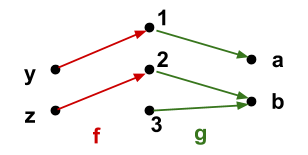
\includegraphics{4.4.4.d}
	
	
\end{list}



%----------------------------------------------------------------------------------------

\end{document}